% MASTER 4 -- Tapered (geometric) cascade of inverters driving a big load C_L.
% Each stage is wider than the previous by the factor b (optimum b = e). Sizes 1, b, b^2, b^3.
% Covers Q3, Q8, Q20 directly. The first TWO triangles also serve as the inverter PAIR (Q12/Q16).
% Total nMOS delay = (N/2)(5 b tau);  N = ln(C_L / squareCg).
\documentclass[border=10pt]{standalone}
\usepackage{tikz}
\usetikzlibrary{arrows.meta}
\begin{document}
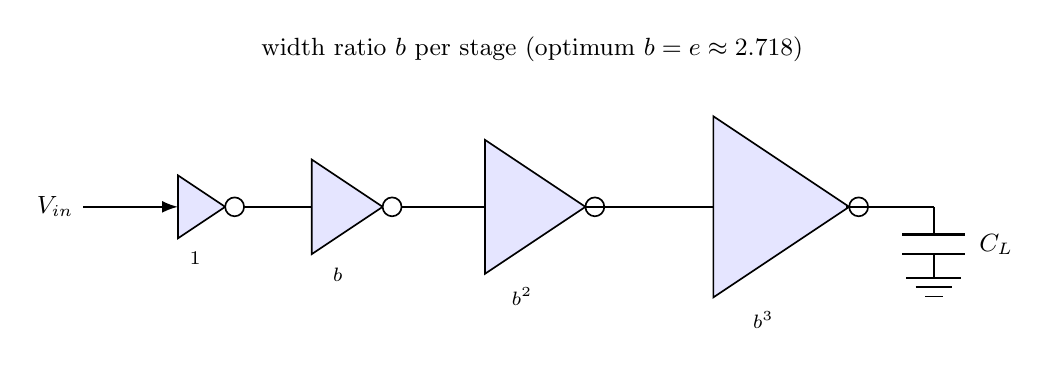
\begin{tikzpicture}[>=Latex,font=\small,line width=0.6pt]
% inverter triangle helper: #1 = left-x, #2 = half-height, #3 = size label
\newcommand{\inv}[3]{%
  \fill[blue!10] (#1,#2) -- (#1,-#2) -- (#1+1.5*#2,0) -- cycle;
  \draw          (#1,#2) -- (#1,-#2) -- (#1+1.5*#2,0) -- cycle;
  \draw[fill=white] (#1+1.5*#2+0.12,0) circle (0.12);
  \node[below] at (#1+0.55*#2,-#2-0.05) {\scriptsize #3};
}
% four inverters of growing size; out_i = leftx + 1.5*h + 0.24
\inv{0}{0.40}{$1$}      % out approx 0.84
\inv{1.7}{0.60}{$b$}    % out approx 2.84
\inv{3.9}{0.85}{$b^2$}  % out approx 5.17
\inv{6.8}{1.15}{$b^3$}  % out approx 8.49
% input
\draw[->] (-1.2,0) node[left]{$V_{in}$} -- (0,0);
% interconnects
\draw (0.84,0) -- (1.7,0);
\draw (2.84,0) -- (3.9,0);
\draw (5.17,0) -- (6.8,0);
\draw (8.49,0) -- (9.6,0) coordinate (cl);
% load capacitor C_L at the end
\draw (cl) -- (9.6,-0.0);
\draw (9.6,0) -- (9.6,-0.35);
\draw[line width=1pt] (9.2,-0.35) -- (10.0,-0.35);
\draw[line width=1pt] (9.2,-0.6)  -- (10.0,-0.6);
\draw (9.6,-0.6) -- (9.6,-0.9);
\draw (9.25,-0.9) -- (9.95,-0.9);
\draw (9.37,-1.02) -- (9.83,-1.02);
\draw (9.49,-1.14) -- (9.71,-1.14);
\node[right] at (10.05,-0.475) {$C_L$};
% caption
\node[align=center] at (4.5,2.0)
  {width ratio $b$ per stage (optimum $b=e\approx2.718$)};
\end{tikzpicture}
\end{document}
